\documentclass{article}
\usepackage{graphicx}
\usepackage{amssymb}
\usepackage{amsmath}
\usepackage{float}
\usepackage{hyperref}
\usepackage{algorithm2e}
\usepackage[margin=1in]{geometry}

\begin{document}

\title{Robotics 811 - Homework 4 - Resubmit}
\author{Xiang Zhi Tan}
\maketitle

\section{Q7}
\subsection*{7(a)}
We can first rearrange the constraints 2 and 3 into the following form by moving elements on the right handside to the left and multiplying constraints 2 by $-1$.
\begin{equation*}
\begin{aligned}
- w^Tx_i - b + 1 - \xi_i &\leq 0\\ \mbox{ if } y_i = 1
w^Tx_i + b + 1 - \xi_i &\leq 0\\ \mbox{ if } y_i = -1
\end{aligned} 
\end{equation*}
Through observing the inequalities, we notice that the only difference is the element $w^Tx_i$ which has a different sign that could be change by the values of $y_i$. This allows us to combine both inequalities into the following constraint.
\begin{equation*}
- y_i(w^Tx_i + b) + 1 - \xi_i \leq = 0
\end{equation*}

\subsection*{7(b)}
The Lagrangian for our optimization problem is as following:
\begin{equation*}
L ([w\;0\;\xi]^T, \alpha, \beta) = \frac{1}{2}||w||^2 + C \sum_{i=1}^l \xi_i + \sum_{i=1}^l \alpha_ig_i([w\;b\;\xi]^T) - \sum_{i=1}^l \beta_i \xi_i
\end{equation*}

\subsection*{7(c)}
Following is the steps to minimize the Lagrangian which is ther primal form of the SVM. Here's the original Lagrangian.
\begin{equation}\label{ori-l}
L ([w\;0\;\xi]^T, \alpha, \beta) = \frac{1}{2}||w||^2 + C \sum_{i=1}^l \xi_i + \sum_{i=1}^l \alpha_i(- y_i(w^Tx_i + b) + 1 - \xi_i) - \sum_{i=1}^l \beta_i \xi_i
\end{equation}
First, we find the partial of $w$,$b$ and $\xi_i$. Following are the partials follow by setting them to 0.\\
Finding partial of $w$
\begin{equation}\label{wpartial}
\begin{aligned}
\frac{\partial}{\partial w} &= \frac{2}{2} w - \sum_{i=1}^l(\alpha_i y_i x_i) = 0\\
w &= \sum_{i=1}^l(\alpha_i y_i x_i)
\end{aligned}
\end{equation}
Finding the partial of $b$.
\begin{equation}\label{bpartial}
\begin{aligned}
\frac{\partial}{\partial b} &= -\sum_{i=1}^l(\alpha_i y_i) = 0\\
\sum_{i=1}^l(\alpha_i y_i) &= 0\\
\end{aligned}
\end{equation}
Finding the partial of $xi_i$.
\begin{equation}\label{xipartial}
\begin{aligned}
\frac{\partial}{\partial \xi_i} &= C - \sum_{i=1}^l(\alpha_i) - \sum_{i=1}^l(\beta_i) = 0\\
C &= \sum_{i=1}^l(\alpha_i) + \sum_{i=1}^l(\beta_i)
\end{aligned}
\end{equation}\tabularnewline
Now we insert equations \ref{wpartial}, \ref{xipartial} in equation \ref{ori-l}.
\begin{equation}
\begin{aligned}
L &= \frac{1}{2}(\sum_{i=1}^l(\alpha_i y_i x_i))^2 + (\sum_{i=1}^l(\alpha_i) + \sum_{i=1}^l(\beta_i))\sum_{i=1}^l \xi_i + \sum_{i=1}^l \alpha_i(- y_i((\sum_{j=1}^l(\alpha_j y_j x_j))x_i + b) + 1 - \xi_i) - \sum_{i=1}^l \beta_i \xi_i\\
L &= \frac{1}{2}(\sum_{i=1}^l\sum_{j=1}^l(\alpha_i \alpha_j y_i y_j x_j^T x_i)) + \sum_{i=1}^l(\alpha_i \xi_i) + \sum_{i=1}^l(\beta_i \xi_i) + \sum_{i=1}^l(\alpha_i \alpha_j y_i y_j x_j^T x_i))\\
&- b \sum_{i=1}^l(\alpha_i y_i) + \sum_{i=1}^l(\alpha_i) - \sum_{i=1}^l(\alpha_i \xi_i) - \sum_{i=1}^l \beta_i \xi_i\\
L &= \sum_{i=1}^l(\alpha_i) - \frac{1}{2}(\sum_{i=1}^l\sum_{j=1}^l(\alpha_i \alpha_j y_i y_j x_j^T x_i)) - b \sum_{i=1}^l(\alpha_i y_i)\\
\end{aligned}
\end{equation}
By applying equation \ref{bpartial} in the previous equation, we can derive the final form
\begin{equation}\label{final-eq}
L^*(\alpha) = \sum_{i=1}^l(\alpha_i) - \frac{1}{2}(\sum_{i=1}^l\sum_{j=1}^l(\alpha_i \alpha_j y_i y_j x_j^T x_i))\\
\end{equation}

\subsection*{7(d)}
As we want to write the equation in terms of $H$ and $f$ such that $L^*(\alpha) = \frac{1}{2} \alpha^TH\alpha + f^T\alpha$. By looking at equation \ref{final-eq}, we see a similar structure between them. For the first part $\frac{1}{2} \alpha^TH\alpha $
\begin{equation*}
\begin{aligned}
\frac{1}{2}\alpha^TH\alpha &= -\frac{1}{2}(\sum_{i=1}^l\sum_{j=1}^l(\alpha_i \alpha_j y_i y_j x_j^T x_i))\\
H &= -(\sum_{i=1}^l\sum_{j=1}^l(y_i y_j x_j^T x_i))
\end{aligned}
\end{equation*}
For second part $f^T\alpha$
\begin{equation*}
\begin{aligned}
f^T\alpha &= \sum_{i=1}^l(\alpha_i)\\
f^T &= [1,1,.....1]
\end{aligned}
\end{equation*}

\subsection*{7(e)(i)}
We implemented the SVM in the matlab file \textbf{svmSolver.m} and the solver can be tested and visualized by the files \textbf{q7e\_1.m} for the first part and \textbf{q7e\_2.m} for the second part of the question.
Following are graphs of using the SVM solver on the test data and the decision boundary and margins for C=1,0.1,0.01.
\begin{figure}[H]
\centering
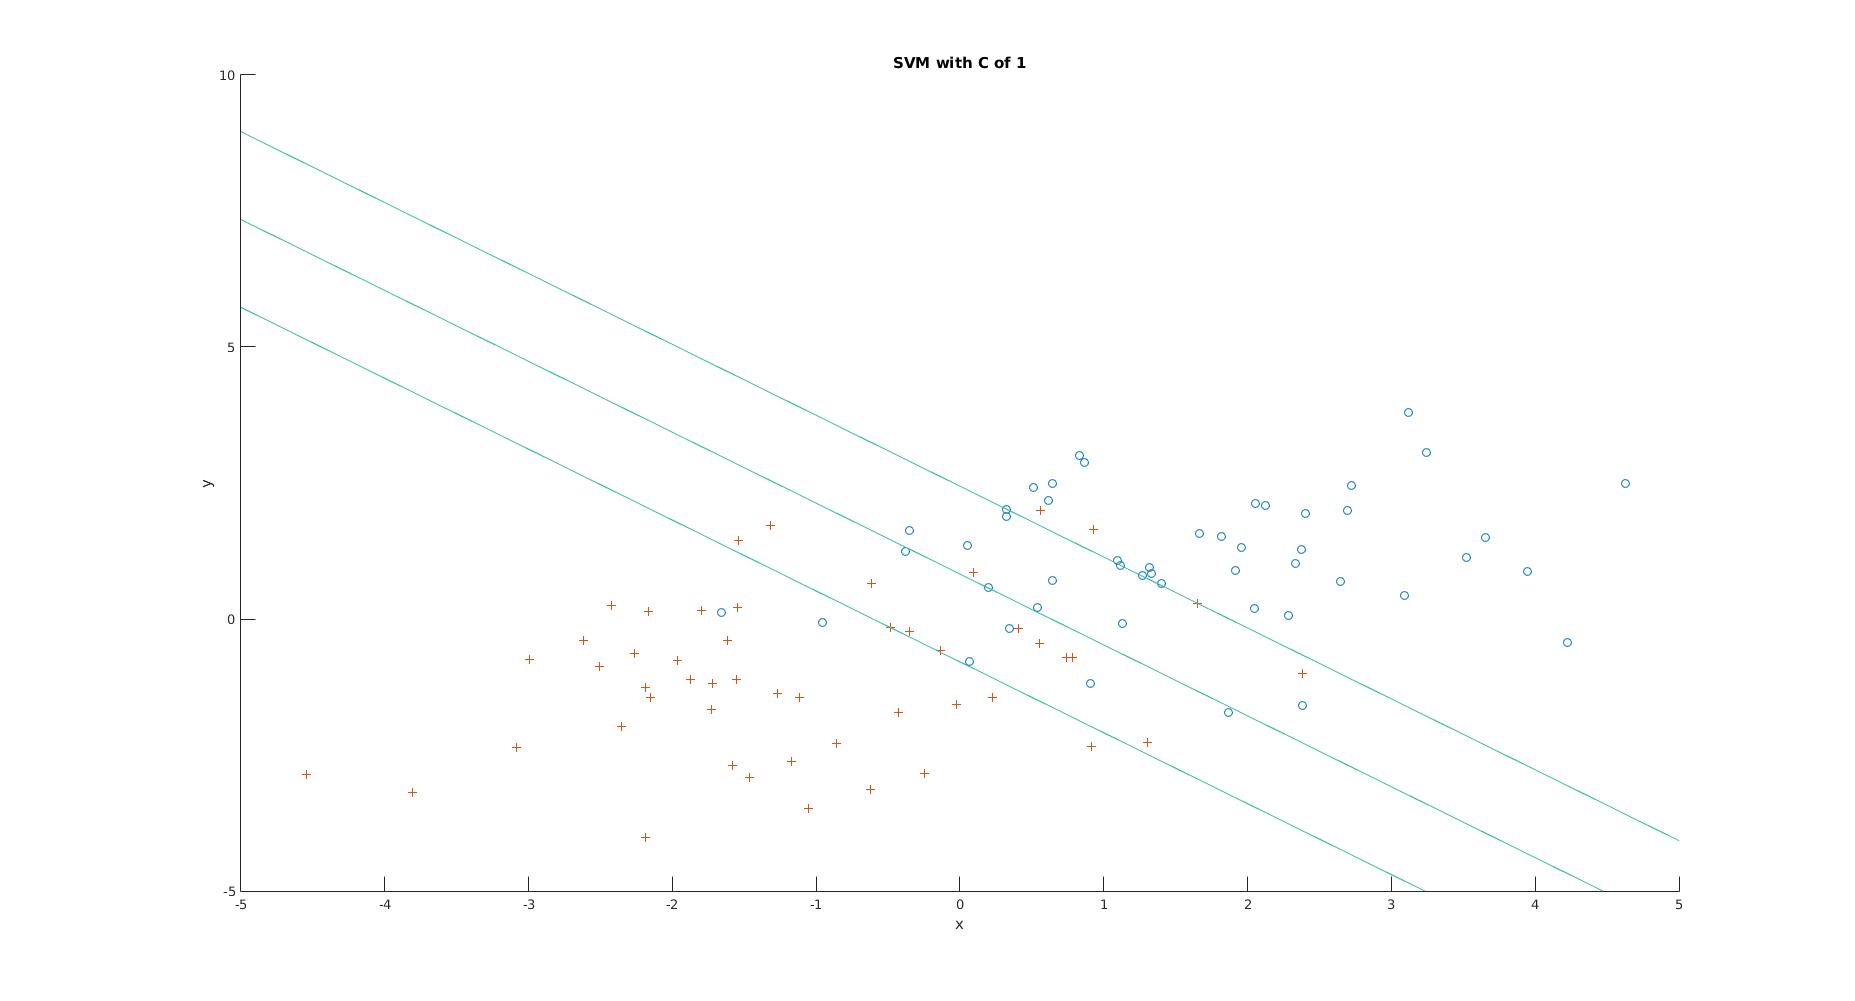
\includegraphics[width=6.5in]{figures/q7-5-3.jpg}
\caption{Plot of decision boundary and margins with C=1}
\end{figure}
\begin{figure}[H]
\centering
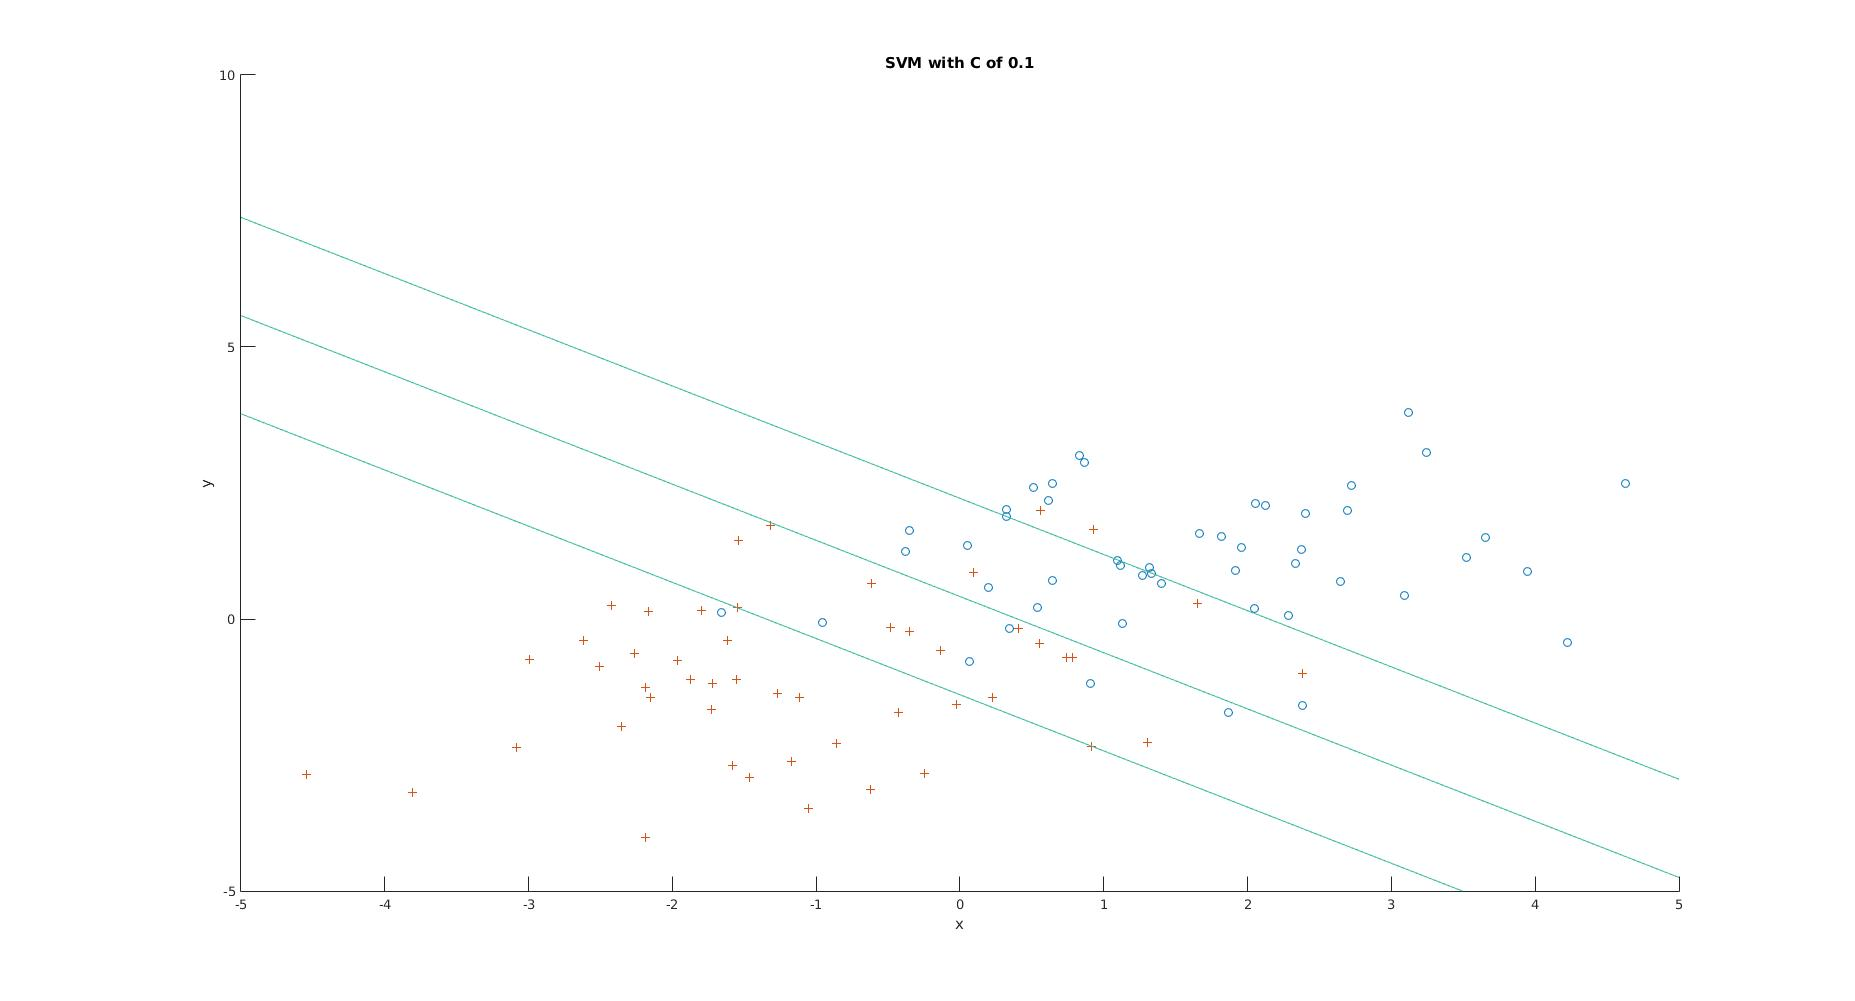
\includegraphics[width=6.5in]{figures/q7-5-2.jpg}
\caption{Plot of decision boundary and margins with C=0.1}
\end{figure}
\begin{figure}[H]
\centering
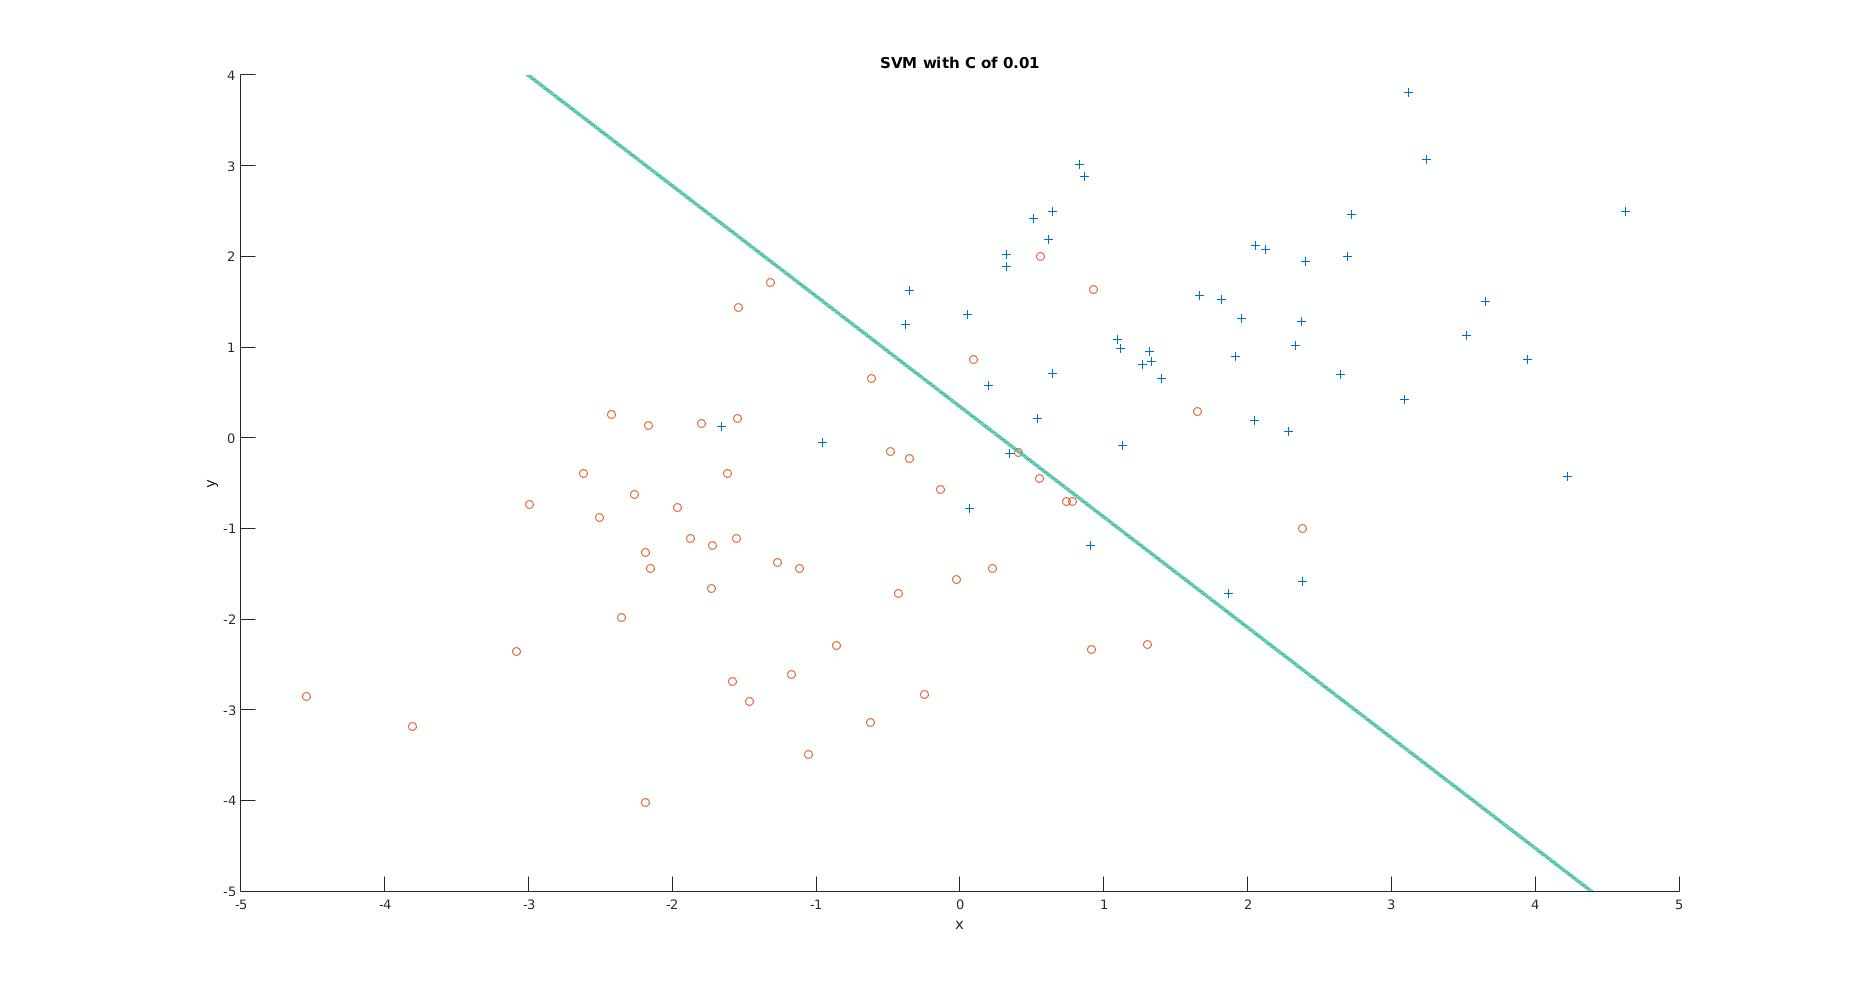
\includegraphics[width=6.5in]{figures/q7-5-1.jpg}
\caption{Plot of decision boundary and margins with C=0.01}
\end{figure}
As C increases, we observe that the locations of the support vector(points that lies on the margin lines) and margin lines gets further away from the decision boundary. This is the expected behavior because the larger the C parameter the more accurate the classification of the training data would be as it tries to create a decision boundary that minimize the training data error but might cause over fitting. Where a smaller C means creating a larger margin that would generalized more to other test sets.

\subsection*{7(e)(ii)}
As observed in the previous few figures, we see that the decision margins increase as C decreases. Therefore, as C approaches $0$, the sampling errors are negated.
\begin{equation}
\lim_{C \to 0} min \frac{1}{2}||w||^2 + C\sum_{i=1}^l\xi_i = min \frac{1}{2}||w||^2
\end{equation}
Therefore, SVM will now ignore the sampling error and might choose points that have significant error as support vectors and give the wrong result 

\subsection*{7(e)(iii)}
This part of the question is implemented in the script,\textbf{q7e\_2.m}.
Following is the table showing the accuracy of my algorithm on a 10-fold cross validation run.\\
\begin{centering}
\begin{tabular}{|c|c|c|c|c|c|c|c|}
\hline
k & correct P & wrongly label & P detection \% & correct N & wrongly label & N detection \% & total accuracy \\ \hline
1 & 122 & 1 & 0.968254 & 126 & 4 & 0.992126 & 0.980237 \\ \hline 
2 & 131 & 0 & 0.970370 & 119 & 4 & 1.000000 &0.984252 \\ \hline 
3 & 122 & 0 & 0.897059 & 117 & 14 & 1.000000& 0.944664 \\ \hline 
4 & 141 & 0 & 0.972414 & 109 & 4 & 1.000000 &0.984252 \\ \hline 
5 & 141 & 0 & 0.979167 & 109 & 3 & 1.000000 &0.988142 \\ \hline 
6 & 129 & 0 & 0.941606 & 117 & 8 & 1.000000 &0.968504 \\ \hline 
7 & 124 & 0 & 0.892086 & 114 & 15 & 1.000000&0.940711 \\ \hline 
8 & 116 & 0 & 0.983051 & 135 & 2 & 1.000000 &0.992095 \\ \hline 
9 & 138 & 0 & 0.992806 & 114 & 1 & 1.000000 &0.996047 \\ \hline 
10 & 133 & 0 & 0.970803 & 117 & 4 & 1.000000 &0.984252 \\ \hline 
\end{tabular}
\caption{The first wrongly label column is the number of N that are labeled as P by the SVM, the second wrongly label column is the number of P that is wrongly label by N by the SVM}
\end{centering}
\\
The average accuracy over the 10 fold validation is $0.9763$ which is pretty good.
\subsection*{7(e)(iv)}
\begin{figure}[H]
\centering
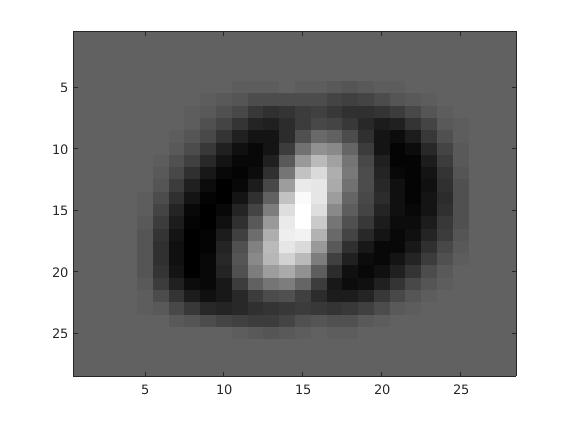
\includegraphics[width=6.5in]{figures/q7-6.jpg}
\caption{plot of weight function}
\end{figure}
The weight functions shows us what the algorithm learns. It assigns mainly positive weights in the center and at the edge in the middle. This shows that for detecting ones, it's important to have pixel values at the corners and the centers which is how a 1 is written. Where a negative weight resemblances a circle around which is the shape of the zeros which is what we are detecting. 
\end{document}